\chapter{$Z \rightarrow \mu^{+}\mu^{-}$ decaying process}
\label{chap:Z}





The process studied in this thesis work is the decay of $Z$ boson, generated by $pp$ collisions, into a pair of muon and antimuon. The scheme of the decay is showed in Figure \ref{fig:Z_MUMU_FEYNMAN}. This is the prevision in the hypothesis of SM, where the $Z$ boson is commonly represented with the symbol $Z^{0}$. The presence of a new physics scenario is modeled by the existence of a new boson, which is commonly indicated in literature with $Z^{\prime}$. In this case, the scheme of the decay is practically similiar and it is showed in Figure \ref{fig:Z_PRIME_FEYNMAN}.

\vspace{5mm}
\begin{minipage}[b]{0.45\linewidth}
    \centering
    \begin{tikzpicture}[scale=1.0]
  		\begin{feynman}
			\node at (0, 0)   (al) {\(p\)};
			\node at (0, -3)	(bl) {\(p\)};
			\node[inner sep=0pt,minimum size=0pt] at (1.5,-1.5)	(dl);
	
			\node at (5, 0)   (ar) {\(\mu^{-}\)};
			\node at (5, -3)	(br) {\(\mu^{+}\)};
			\node[inner sep=0pt,minimum size=0pt] at (3.5,-1.5)	(dr);
 
    		\diagram* {
      		(al) -- [fermion] (dl) -- [fermion] (bl),
      		(dl) -- [cyan, boson, edge label'=\(\color{black}Z^{0}/\gamma^{*}\)] (dr),
      		(ar) -- [anti fermion] (dr) -- [anti fermion] (br)
    		};
  		\end{feynman}
	\end{tikzpicture}
    \captionof{figure}{$Z$ decay in the hypotesis of SM.}
    \label{fig:Z_MUMU_FEYNMAN}
\end{minipage}
%
\hspace{2mm}
%
\begin{minipage}[b]{0.45\linewidth}
    \centering
    \begin{tikzpicture}[scale=1.0]
  		\begin{feynman}
			\node at (0, 0)   (al) {\(p\)};
			\node at (0, -3)	(bl) {\(p\)};
			\node[inner sep=0pt,minimum size=0pt] at (1.5,-1.5)	(dl);
	
			\node at (5, 0)   (ar) {\(\mu^{-}\)};
			\node at (5, -3)	(br) {\(\mu^{+}\)};
			\node[inner sep=0pt,minimum size=0pt] at (3.5,-1.5)	(dr);
 
    		\diagram* {
      		(al) -- [fermion] (dl) -- [fermion] (bl),
      		(dl) -- [cyan, boson, edge label'=\(\color{black}Z^{\prime}/\gamma^{*}\)] (dr),
      		(ar) -- [anti fermion] (dr) -- [anti fermion] (br)
    		};
  		\end{feynman}
	\end{tikzpicture}
    \captionof{figure}{$Z^{\prime}$ decay in the new physics scenario.}
    \label{fig:Z_PRIME_FEYNMAN}
\end{minipage}
\vspace{5mm}

The new physics process can by studied by searching for resonant phenomena, for example bumps in the distributions of a set of observables in a zone where only background is expected to be present. However, this is not the only case possible in the wide variety of new physics scenarios. In fact, the existence of new phenomena could not lead to a resonant peak in the distribution of the high level features, but in general to a different shape in the same distributions. For example, there could be a different slope in the exponential falling distribution of background events in the SM hypothesis.

Neural Networks can be employed in both cases, in general with different performances. The purpose of this thesis work will focus mainly on the new physics scenario of resonant phenomena.

In the following discussion, the $Z^{0}$ boson will be generally described along with its properties and the features employed for the purpose of this work are presented with plots of their distribution.





\section{The $Z^{0}$ boson}
% https://home.cern/science/physics/z-boson
% https://atlas.physicsmasterclasses.org/en/zpath_lhcphysics2.htm
The $Z$ boson is an elementary particle which is the carrier of the weak force, along with the $W$ boson. The difference with the ladder is that while the $W$ boson is charged, the $Z$ boson is neutral. It was discovered in 1983 at CERN at the Super Proton Synchrotron.

Since $Z$ is neutral, the sum of the charges of its decay products must be 0 for the conservation of charge. So it goes without saying that $Z$ must decay into a pair of a particle and its antiparticle. There are several possibilities for the decay process\footnotemark:
\begin{itemize}
	\item In 10\% of $Z$ decays charged lepton-antilepton pairs are produced. Therefore there are three sub-cases for the pairs:
	\begin{itemize}
		\item[$\triangleright$] electron-positron;
		\item[$\triangleright$] muon-antimuon;
		\item[$\triangleright$] tau-antitau;
	\end{itemize}
	
	\item In 20\% of cases it decays into a neutrino-antineutrino pair. However, they are invisible to the detector since they don't interact with anything, in fact they have no charge. A way to indirectly detect their presence is to check if there is some energy or transverse momentum missing after the collision. There are three possibilities for neutrino decay as well as for the pair of leptons.
	
	\item In 70\% of cases the decay gives a quark-antiquark pair. These appear as particle showers called `jets' in the detector. Concerning the possibilities for this mode of decay, quarks appear in six different types (up, down, charm, strange, top, bottom) and three different `colours'. Therefore there are 18 possibilities for the quark-antiquark pair decay.
\end{itemize}

\footnotetext{The information on the fractions of decay can be found in \cite{zboson}}

The set of possible cases counts 24 possibilities, 21 of which are visible. In this work only one will be considered, i.e. the muon-antimuon decay.





\section{High-Level Features for $\mu^{+}\mu^{-}$ decay analysis}
The raw data taken by the detector after the collision is a set of low-level features, briefly LLFs, such as the muon and antimuon momenta. Since we are trying to understand the process in three dimensions with one of the axes aligned with the $y$ component of the first muon, the LLFs of interest are $p_{1,x}$, $p_{1,z}$, $p_{2,x}$, $p_{2,y}$, $p_{2,z}$
To better study the decaying process, it is preferred to combine the low level features into the high-level ones, briefly HLFs.

\begin{table}[H]
	\begin{center}
		\begin{tabular}{c c}
			\toprule
			\toprule
			Symbol	&	HLF name	\\
			\midrule
			$p_{T,1}$		&	Transverse momentum 1			\\
			$p_{T,2}$		&	Transverse momentum 2			\\
			$\eta_{1}$		&	Pseudorapidity 1				\\
			$\eta_{2}$		&	Pseudorapidity 2				\\
			$\Delta \phi$	&	Difference of azimuthal angles	\\
			$M_{Z}$			&	Invariant mass					\\
			\bottomrule
			\bottomrule
		\end{tabular}
		\caption{High Level Features legend.}
		\label{tab:HLF}
	\end{center}
\end{table}

The relations employed to obtain the values for the HLFs are reported in the Equations \ref{eqn:P_T_1}-\ref{eqn:INV_MASS}. The intermediate steps to get the results are reported as well for completeness\footnotemark.
\footnotetext{Note that although the polar angle $\theta$ is a HLF too, the pseudorapidiy is a more common variable and so its usage is preferred in High-Energy Physics.}

\begin{align}
	p_{T,1} &= p_{1,x}	\label{eqn:P_T_1}	\\
	p_{T,2} &= \sqrt{ p_{2,x}^2 + p_{2,y}^2 }	\label{eqn:P_T_2}	\\
	\eta_{1} &= \arctanh{ \left( \frac{p_{1,z}}{p_{1}} \right) }	\label{eqn:PR_1}	\\
	\eta_{2} &= \arctanh{ \left( \frac{p_{2,z}}{p_{2}} \right) }	\label{eqn:PR_2}	\\
	\Delta \phi &= \phi_{2} - \phi_{1}	\label{eqn:DELTA_PHI}	\\
	M_{Z}^{2} &= 2 p_{T,1} p_{T,2} [ \cosh{(\eta_{1} - \eta_{2})} - \cos{\Delta \phi} ]	\label{eqn:INV_MASS}
\end{align}

\noindent
where:

\begin{align}
	p_{1} &= \sqrt{ p_{1,x}^2 + p_{1,z}^2 }	\\
	p_{2} &= \sqrt{ p_{2,x}^2 + p_{2,y}^2 + p_{2,z}^2 }	\\
	\phi_{1} &= \arccos{ \left( \frac{p_{1,x}}{p_{T,1}} \right) }	\\
	\phi_{2} &= \sign{(p_{2,y})} \arccos{ \left( \frac{p_{2,x}}{p_{T,2}} \right) } + \pi [1 - \sign{(p_{2,y})}]
\end{align}





\section{The datasets analyzed}
In order to build an analysis strategy and perform a test of its performances, two benchmark datasets were simulated and for each of them another dataset containing signal events beyond SM was generated. This phase was accomplished through the aid of the framework \textsc{MadGraph5}, assuming $pp$ collisions at $\sqrt{s} = 13~\si{TeV}$. The detector response was also taken into account by \textsc{Delphes}, showering and hadronization by \textsc{Pythia}. More informations on these softwares and on their usage can be found in \cite{madgraph}.

A brief description of the two models studied is given:
\begin{itemize}
	\item The first dataset, denoted with \textbf{Zmumu-Zprime}, is characterized by:
	\begin{itemize}
		\item[$\triangleright$] A `reference' subset following a model with a Breit-Wigner invariant mass distribution, so with a resonant peak at $M_{Z} \approx 91~\si{GeV}$, due to the $Z$ boson.
		\item[$\triangleright$] A `signal' subset whose invariant mass distribution exhibits a resonant peak at $M_{Z} \approx 300~\si{GeV}$.
	\end{itemize}
	
	\item The second dataset, denoted with \textbf{EFT\_YW06}, is characterized by:
	\begin{itemize}
		\item[$\triangleright$] a `reference' subset following a model with a power-law descending invariant mass distribution with a resonant peak at $M_{Z} \approx 91~\si{GeV}$, due to the $Z$ boson.
		\item[$\triangleright$] a `signal' subset whose invariant mass distribution is equal to the reference one, except for a different slope in the power-law descent.
	\end{itemize}
	The tag given to this dataset indicates an Effective Field Theory where the Yukawa coefficient is set to 0 for both signal and reference subsets and Wilson coefficient is set to 0 for reference and to $10^{-6}$ for signal subset. The electomagnetic coupling term $\alpha$ is set to $\approx 1/127.9$ for both subsets.
\end{itemize}

For every case presented, the HLFs were extrapolated by the five independent momenta components. The distributions of the features are showed in following plots, in Figure \ref{fig:Z_PRIME_FEATURES_DISTRIBUTIONS} for \textbf{Zmumu-Zprime} and in Figure \ref{fig:EFT_YW06_FEATURES_DISTRIBUTIONS} for \textbf{EFT\_YW06}.

% **************************************************************
\begin{comment}
\begin{figure}
	\begin{center}
		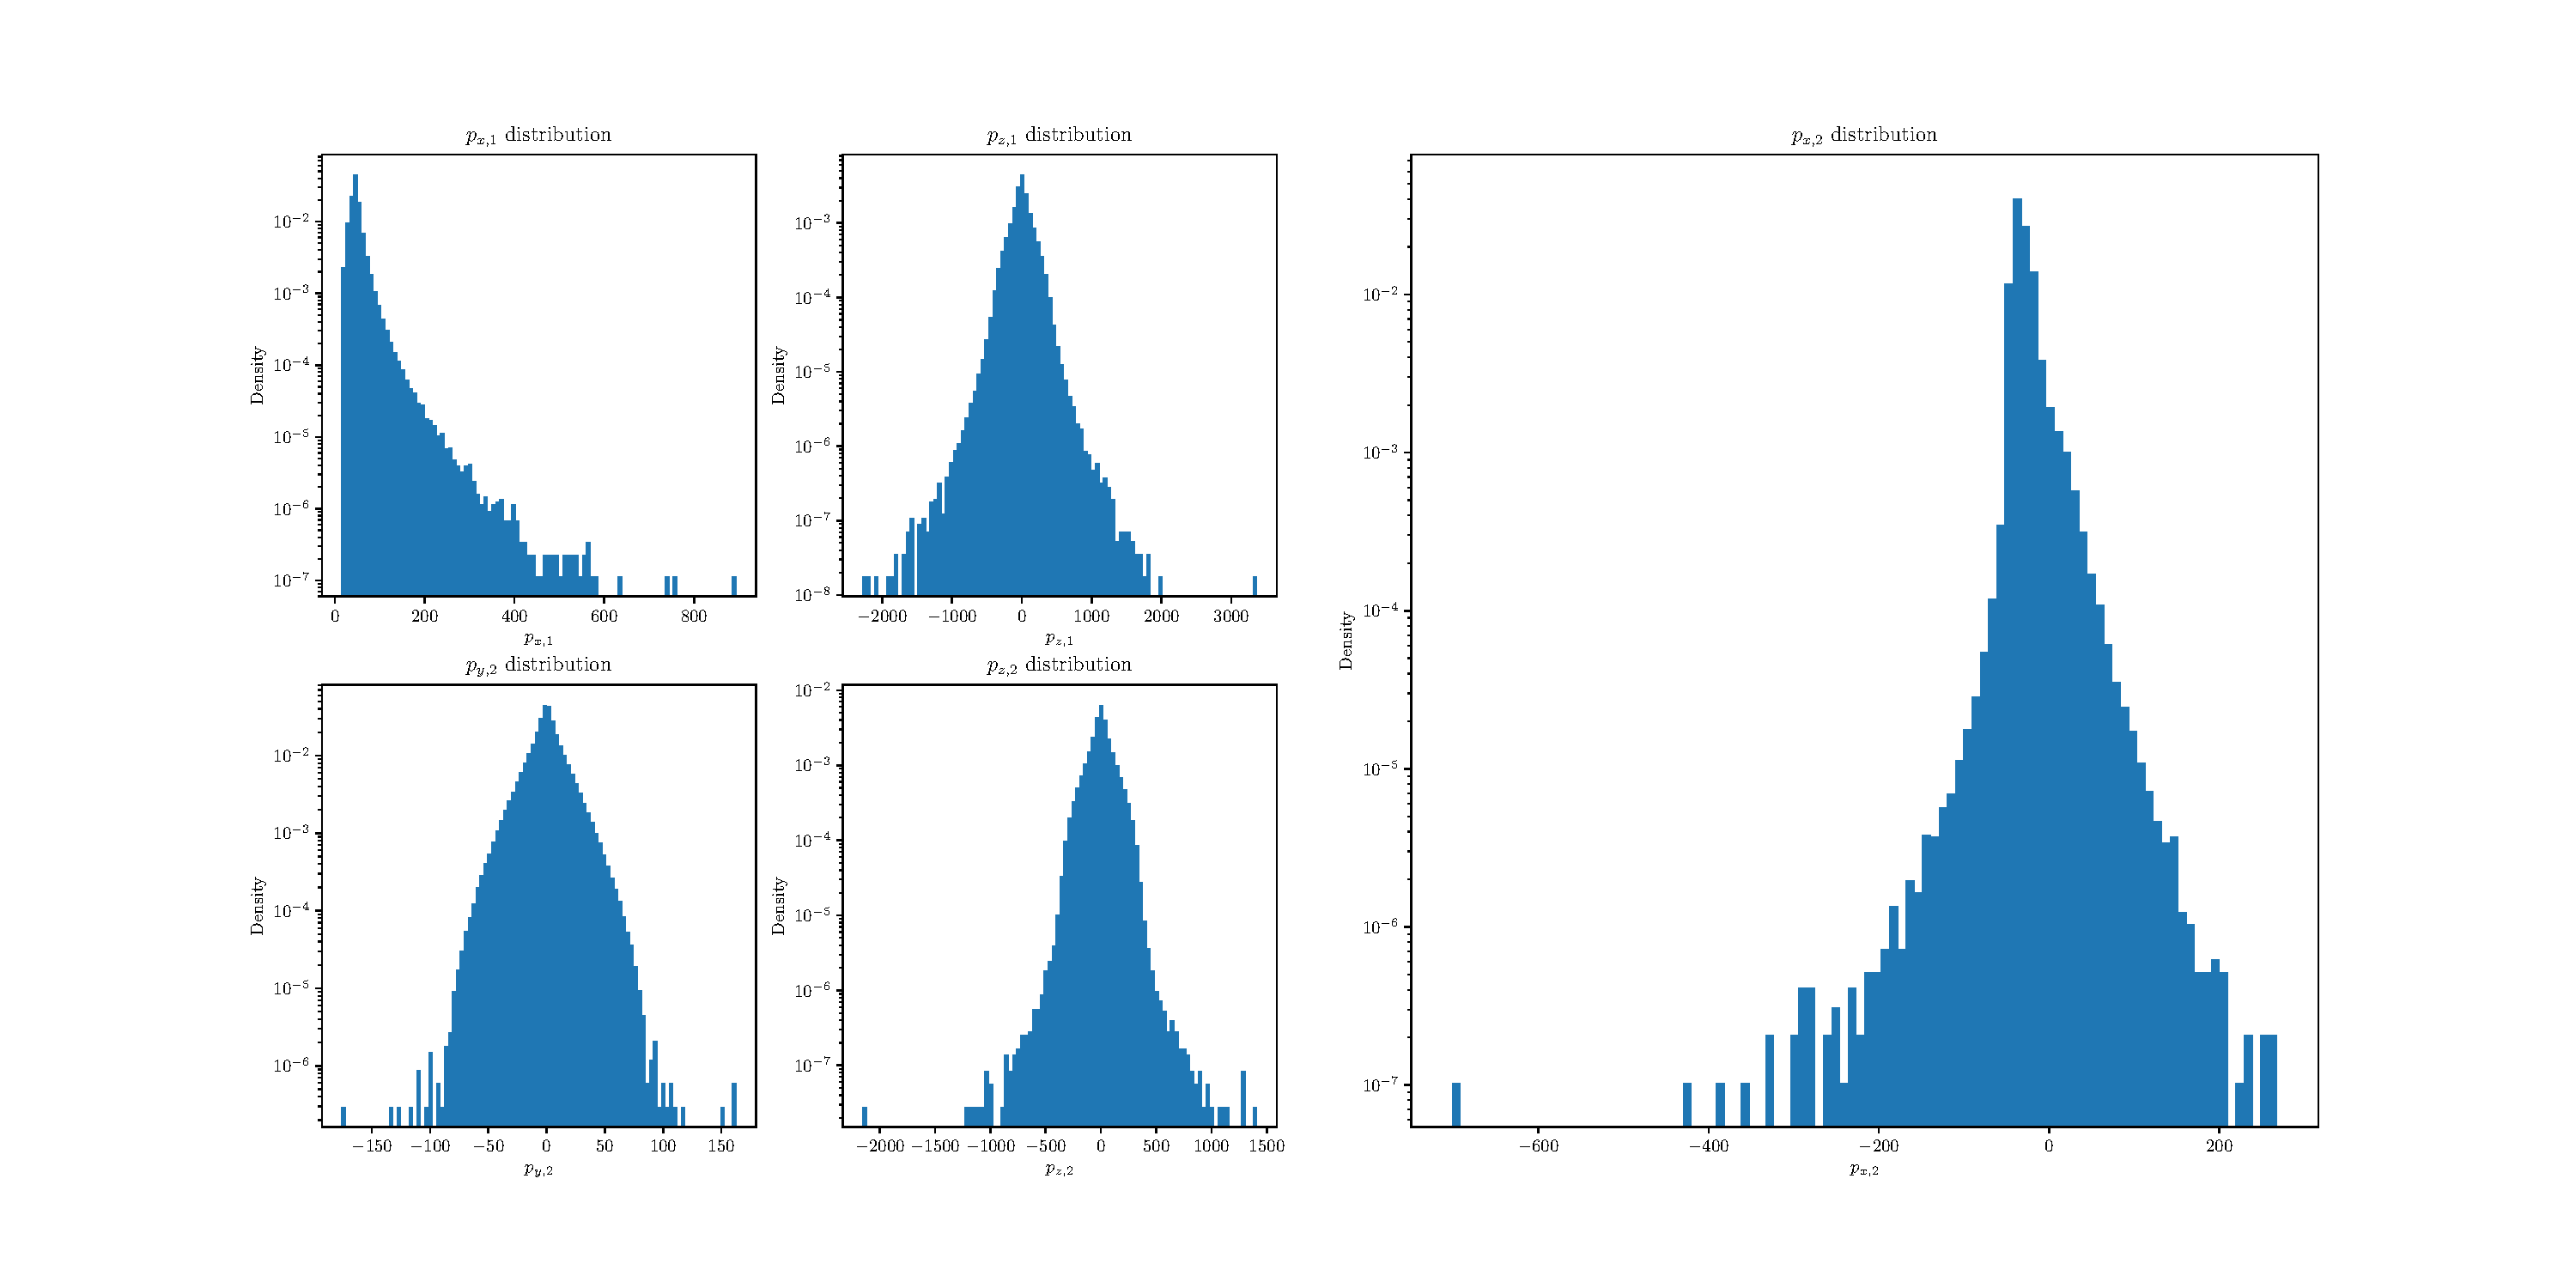
\includegraphics[width=1.0\textwidth]{Python/Z/data.pdf}
		\caption{Data distribution.}
		\label{fig:DATA_DISTRIBUTIONS}
	\end{center}
\end{figure}
\end{comment}
% **************************************************************

\begin{figure}
	\centering
	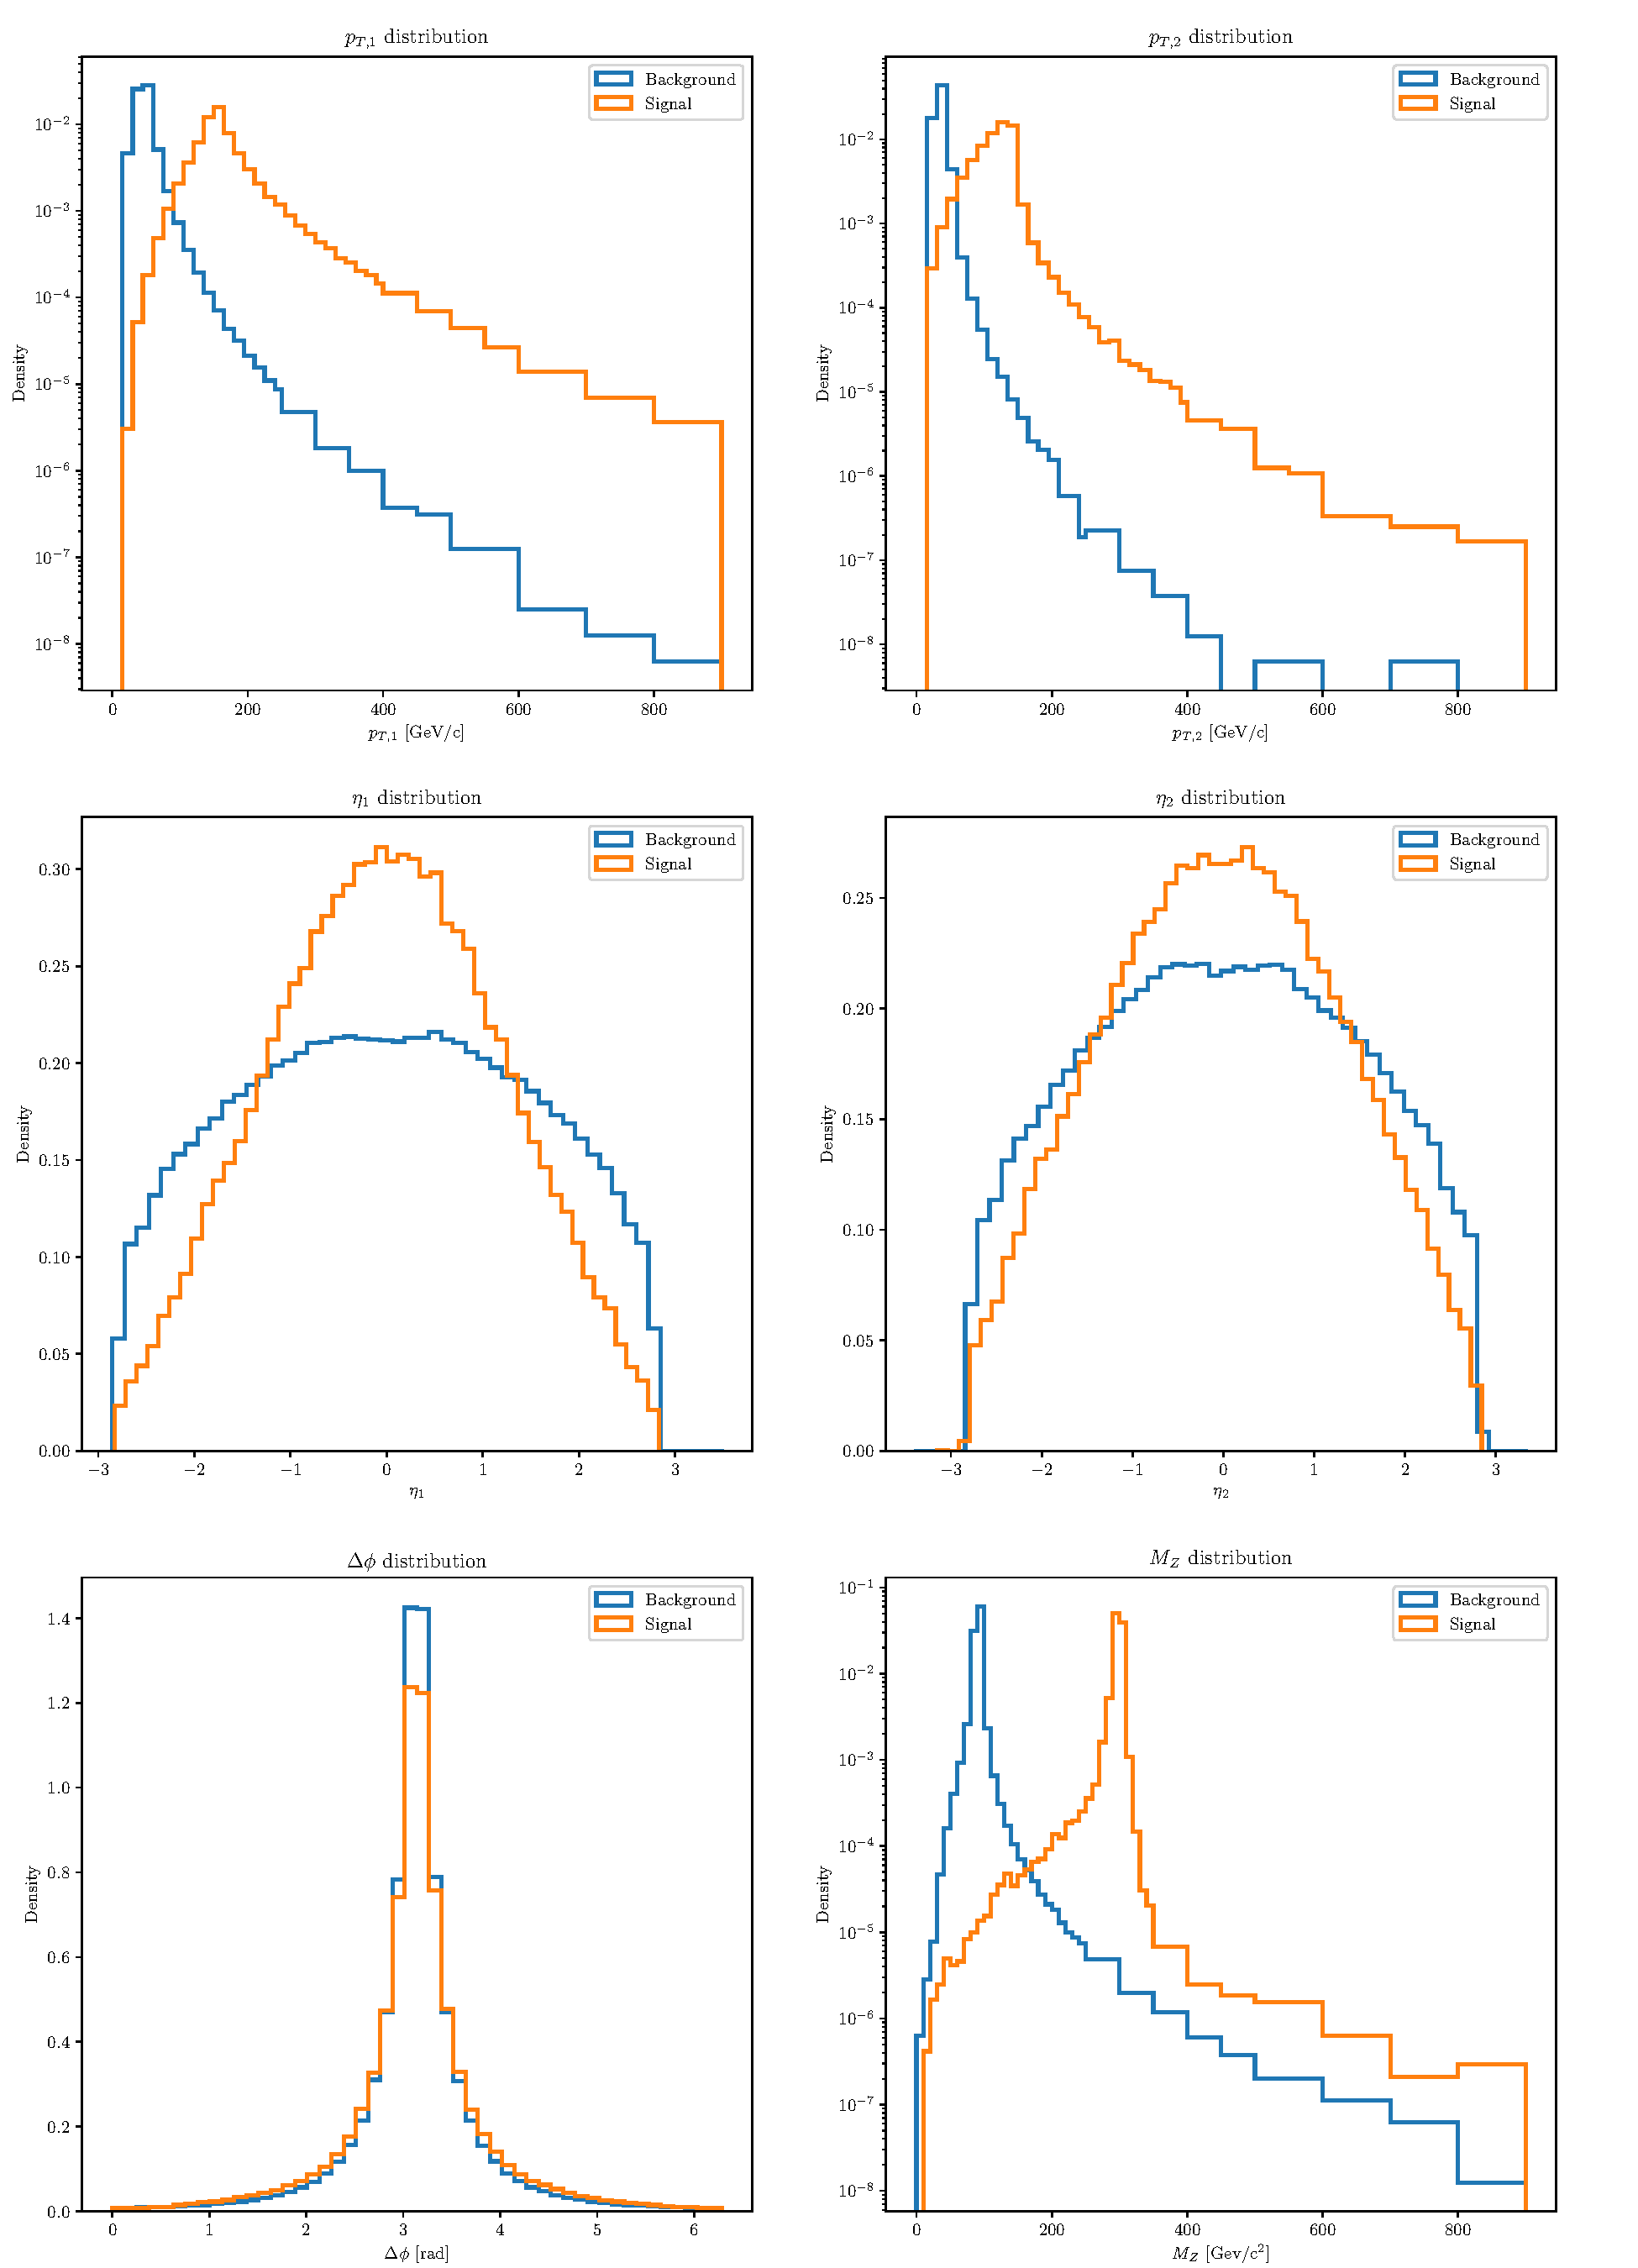
\includegraphics[width=1.0\textwidth]{Python/Z/features_Zmumu_Zprime.pdf}
	\caption{Distributions of the features for \textbf{Zmumu-Zprime}.}
	\label{fig:Z_PRIME_FEATURES_DISTRIBUTIONS}
\end{figure}

\begin{figure}
	\centering
	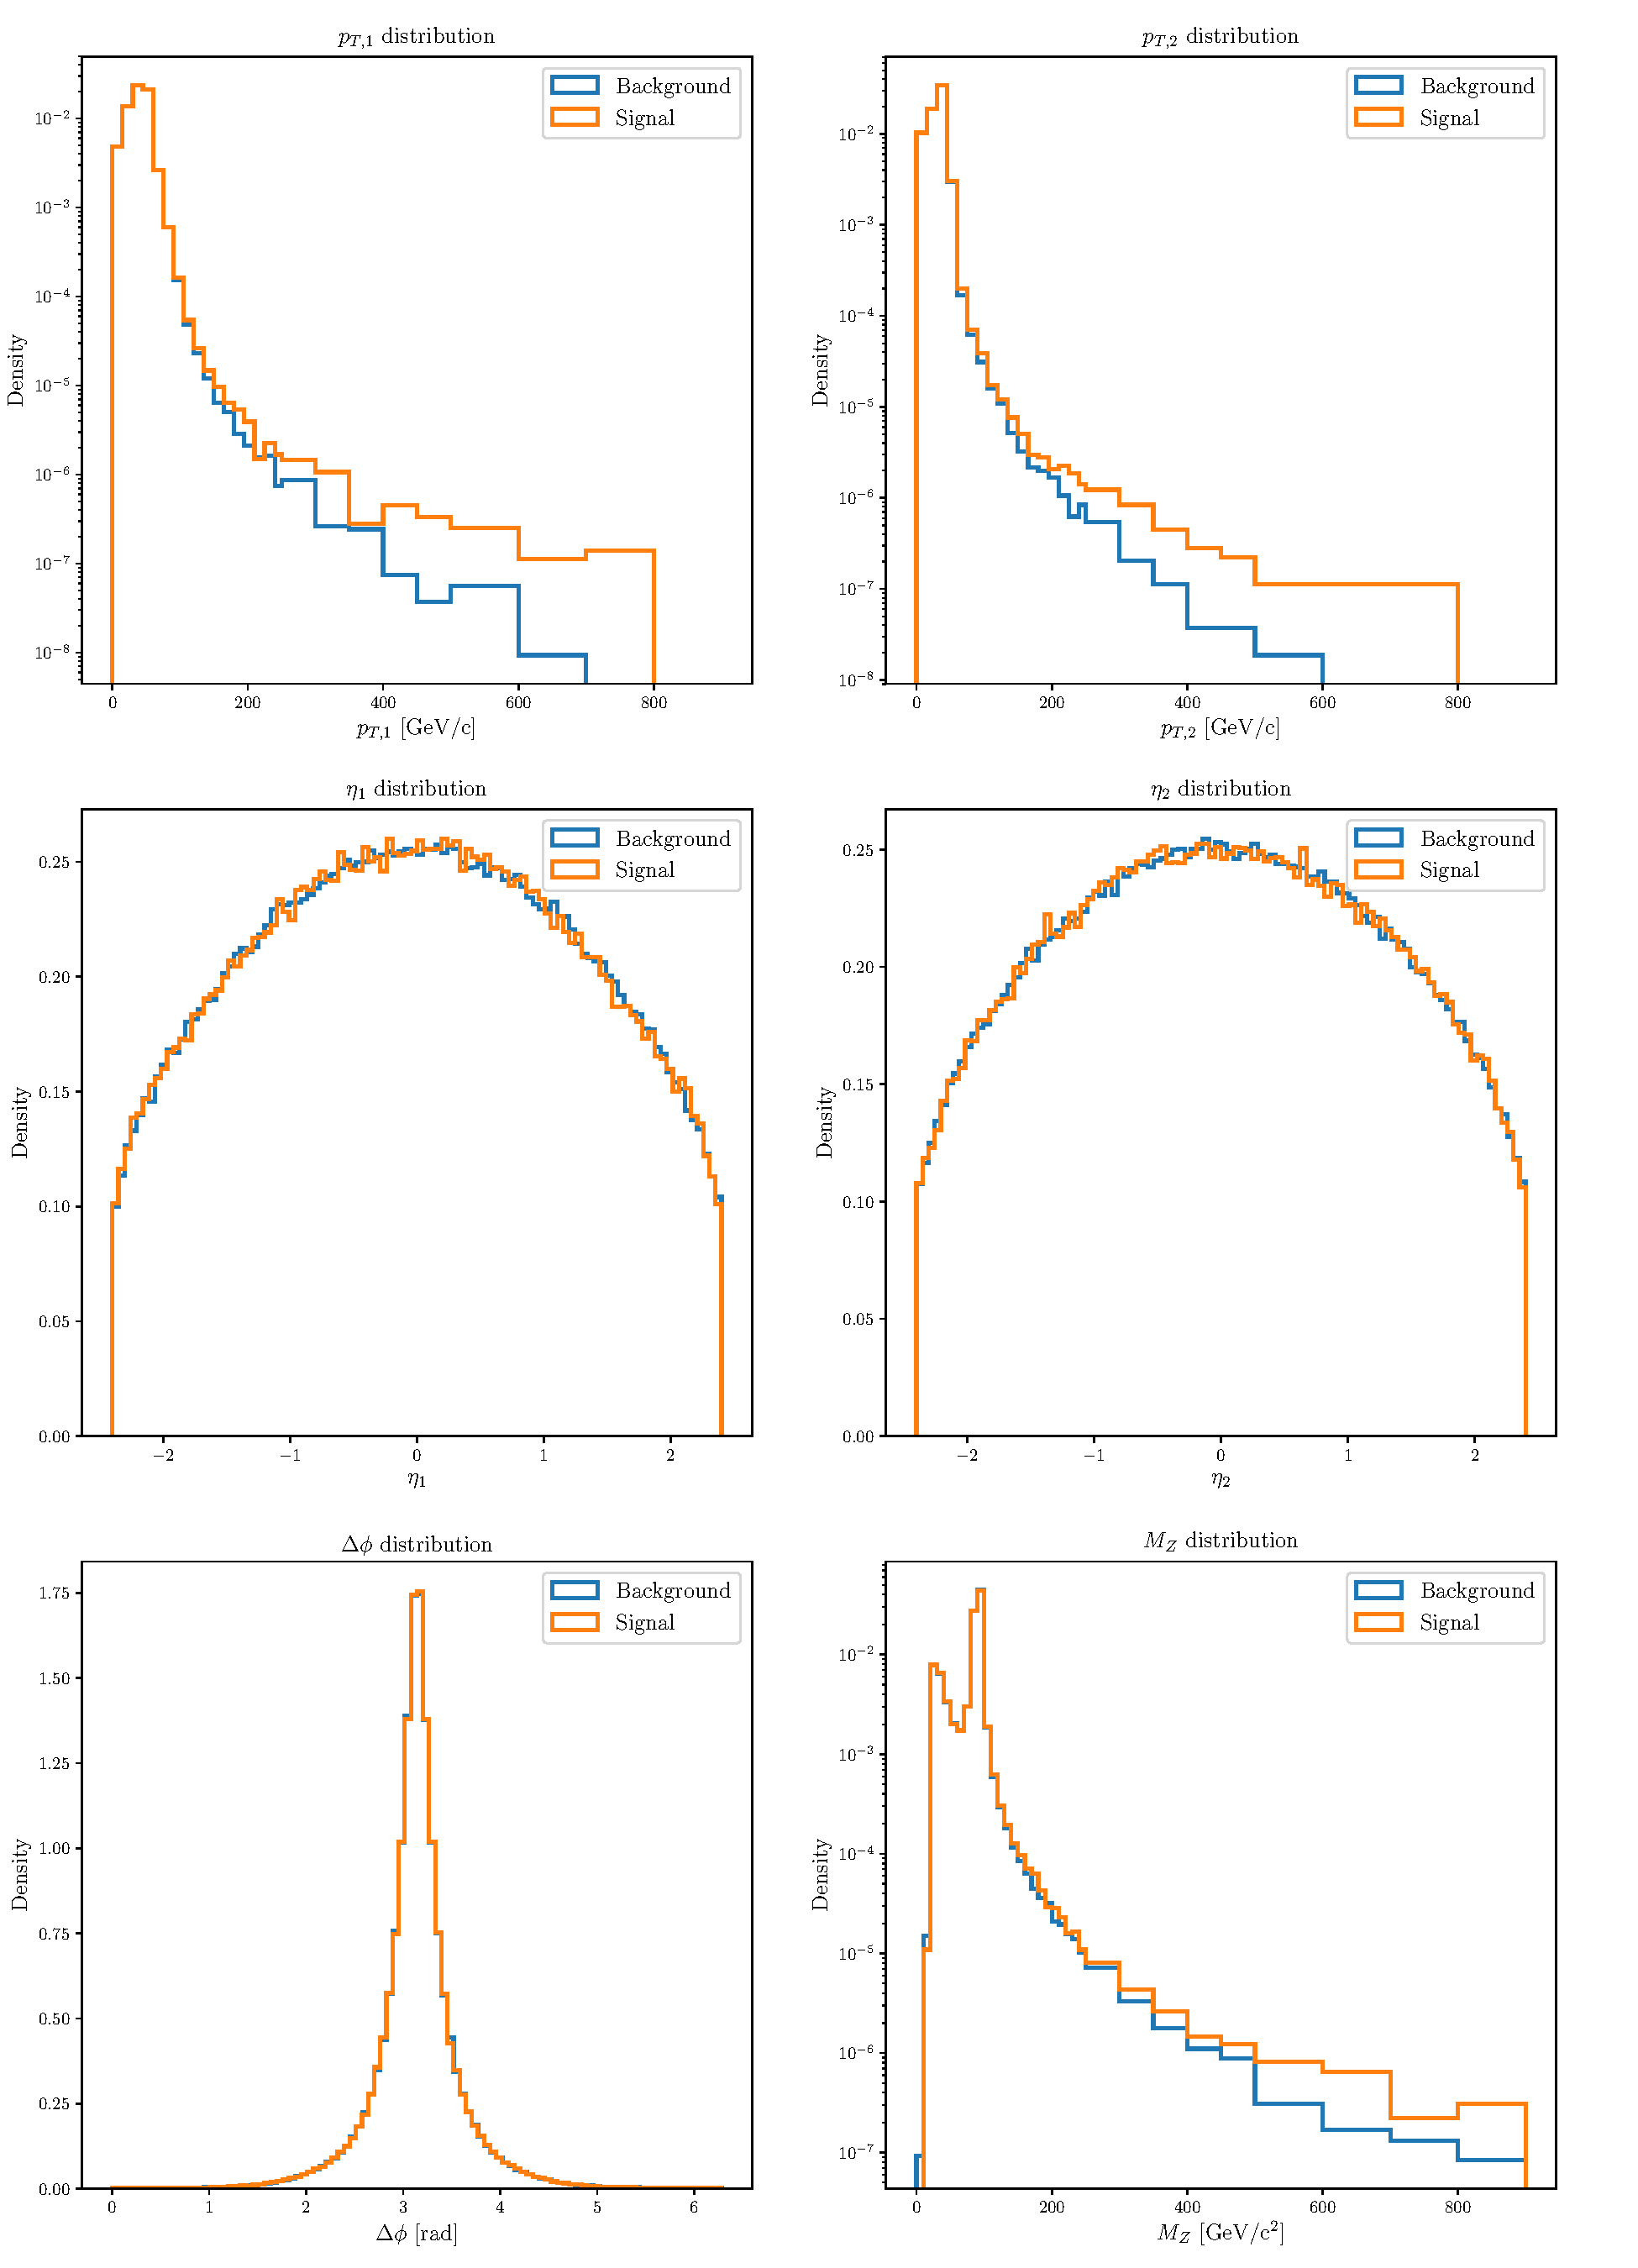
\includegraphics[width=1.0\textwidth]{Python/Z/features_EFT_YW06.pdf}
	\caption{Distributions of the features for \textbf{EFT\_YW06}.}
	\label{fig:EFT_YW06_FEATURES_DISTRIBUTIONS}
\end{figure}